\documentclass[11pt,a4paper]{article}
\usepackage[hyperref]{acl2020}
\usepackage{times}
\usepackage{latexsym}
\usepackage{graphicx}
\renewcommand{\UrlFont}{\ttfamily\small}

\usepackage{microtype}

\aclfinalcopy

\newcommand\BibTeX{B\textsc{ib}\TeX}

\title{Tutela: An Anonymity Tool for Ethereum and Tornado Cash}

\author{
  \small{Mike Wu, Will McTighe, Kaili Wang}\\
  \small{Stanford University} \\ \And
  \small{Nick Bax} \\
  \small{Convex Research} \\ \And
  \small{Istv\'{a}n A. Seres} \\
  \small{E\"{o}tv\"{o}s Lor\'{a}nd University} \\ \AND
  \small{Frederico Carrone, Tomas De Mattey, Manuel Puebla, Herman O. Demaestri, Mariano Nicolini, Pedro Fontana} \\
  \small{LambdaClass} \\}
\date{}

\begin{document}
\maketitle
\begin{abstract}
A common misconception among blockchain users is that decentralization guarantees privacy. The reality is almost the opposite as every transaction one makes, being recorded on a public ledger, reveals information about one's identity.
Mixers, such as Tornado Cash, were developed to preserve privacy through ``mixing'' transactions in an anonymity pool, such that it is impossible to identify who withdrew tokens from the pool. Unfortunately, it is still possible to reveal information about those in the anonymity pool if users are not careful.
We introduce Tutela, an application built on expert heuristics to report the true anonymity of an Ethereum address.
In particular, Tutela has two functionalities: first, it clusters together Ethereum addresses based on interaction history such that for an Ethereum address, we can identify other addresses likely owned by the same entity; second, Tutela computes the true size of the anonymity pool of Tornado Cash mixing, taking into account compromised addresses that reveal identity information. A public implementation of Tutela can be found at \url{https://github.com/TutelaLabs/tutela-app}.
\end{abstract}

\section{Introduction}

On any modern blockchain, the cost of creating a new wallet, being virtually zero, enables the same entity to manage several pseudonymous addresses. The decentralization underpinning blockchains like Bitcoin \citep{nakamoto2008bitcoin} and Ethereum \citep{buterin2013ethereum}, breeds a sense of privacy. This often leads to misuse \citep{christin2013traveling}, such as money laundering through a large number of addresses \citep{moser2013inquiry}, or unfair voting power distributed among multiple addresses owned by the same user. Thus, it is of interest in many investigations to identify addresses linked to the same entity. This is predominantly done through heuristics. Every transaction an address makes on the blockchain, being a public ledger, reveals information about the underlying entity. As such, with graph analysis tools, one can cluster addresses together that with reasonable confidence, possess the same owner.

Such anonymity tools have been widely explored for Bitcoin \cite{haslhofer2016bitcoin,kappos2018empirical}, leveraging heuristics targeting the unspent transaction (UTXO) model. However, this has limited application to more recent blockchain implementations like Ethereum, that forgo the UTXO model for a smart contract model.
Ethereum, in particular, has an account-based protocol that implicitly encourages an entity to reuse a handful of addresses.
As such, this poses greater challenges to user privacy than UTXO-based blockchains.

In response to this shortcoming, several coin mixing protocols have been proposed like M\"{o}bius \citep{meiklejohn2018mobius}, MixEth \citep{seres2019mixeth}, and Tornado Cash \citep{pertsev2019tornado} to obfuscate transaction tracing, the final of which is deployed in practice.
 % As this has limited application to more recent blockchains like Ethereum, new heuristics \citep{victor2020address,beres2021blockchain} have surfaced focusing on graph analysis of transactions between addresses.
Still, new heuristics have surfaced \citep{victor2020address,beres2021blockchain} that deanonymize Ethereum users. These heuristics largely exist in academic silos, and not been combined nor demonstrated in application.

Our primary contribution is the development of a web application that combines several state-of-the-art heuristics to measure the anonymity of Ethereum addresses. In doing so, we create a rich depiction of user behavior and privacy.
We also propose a set of new heuristics targeted at Tornado Cash, motivating that careless user behavior, despite using a mixer, can still reveal identity. The remainder of this whitepaper discusses the heuristics and engineering underlying the web application. A Python implementation is open sourced at \url{https://github.com/TutelaLabs/tutela-app}.

\section{Tutela Overview}

Tutela\footnote{At the time of publication, Tutela is hosted at \url{https://www.tutela.xyz}.}, latin for protection, is a web application that informs users which of their Ethereum addresses are affiliated. Users can search an address, and receive a summary of their anonymity.

\begin{figure}[h!]
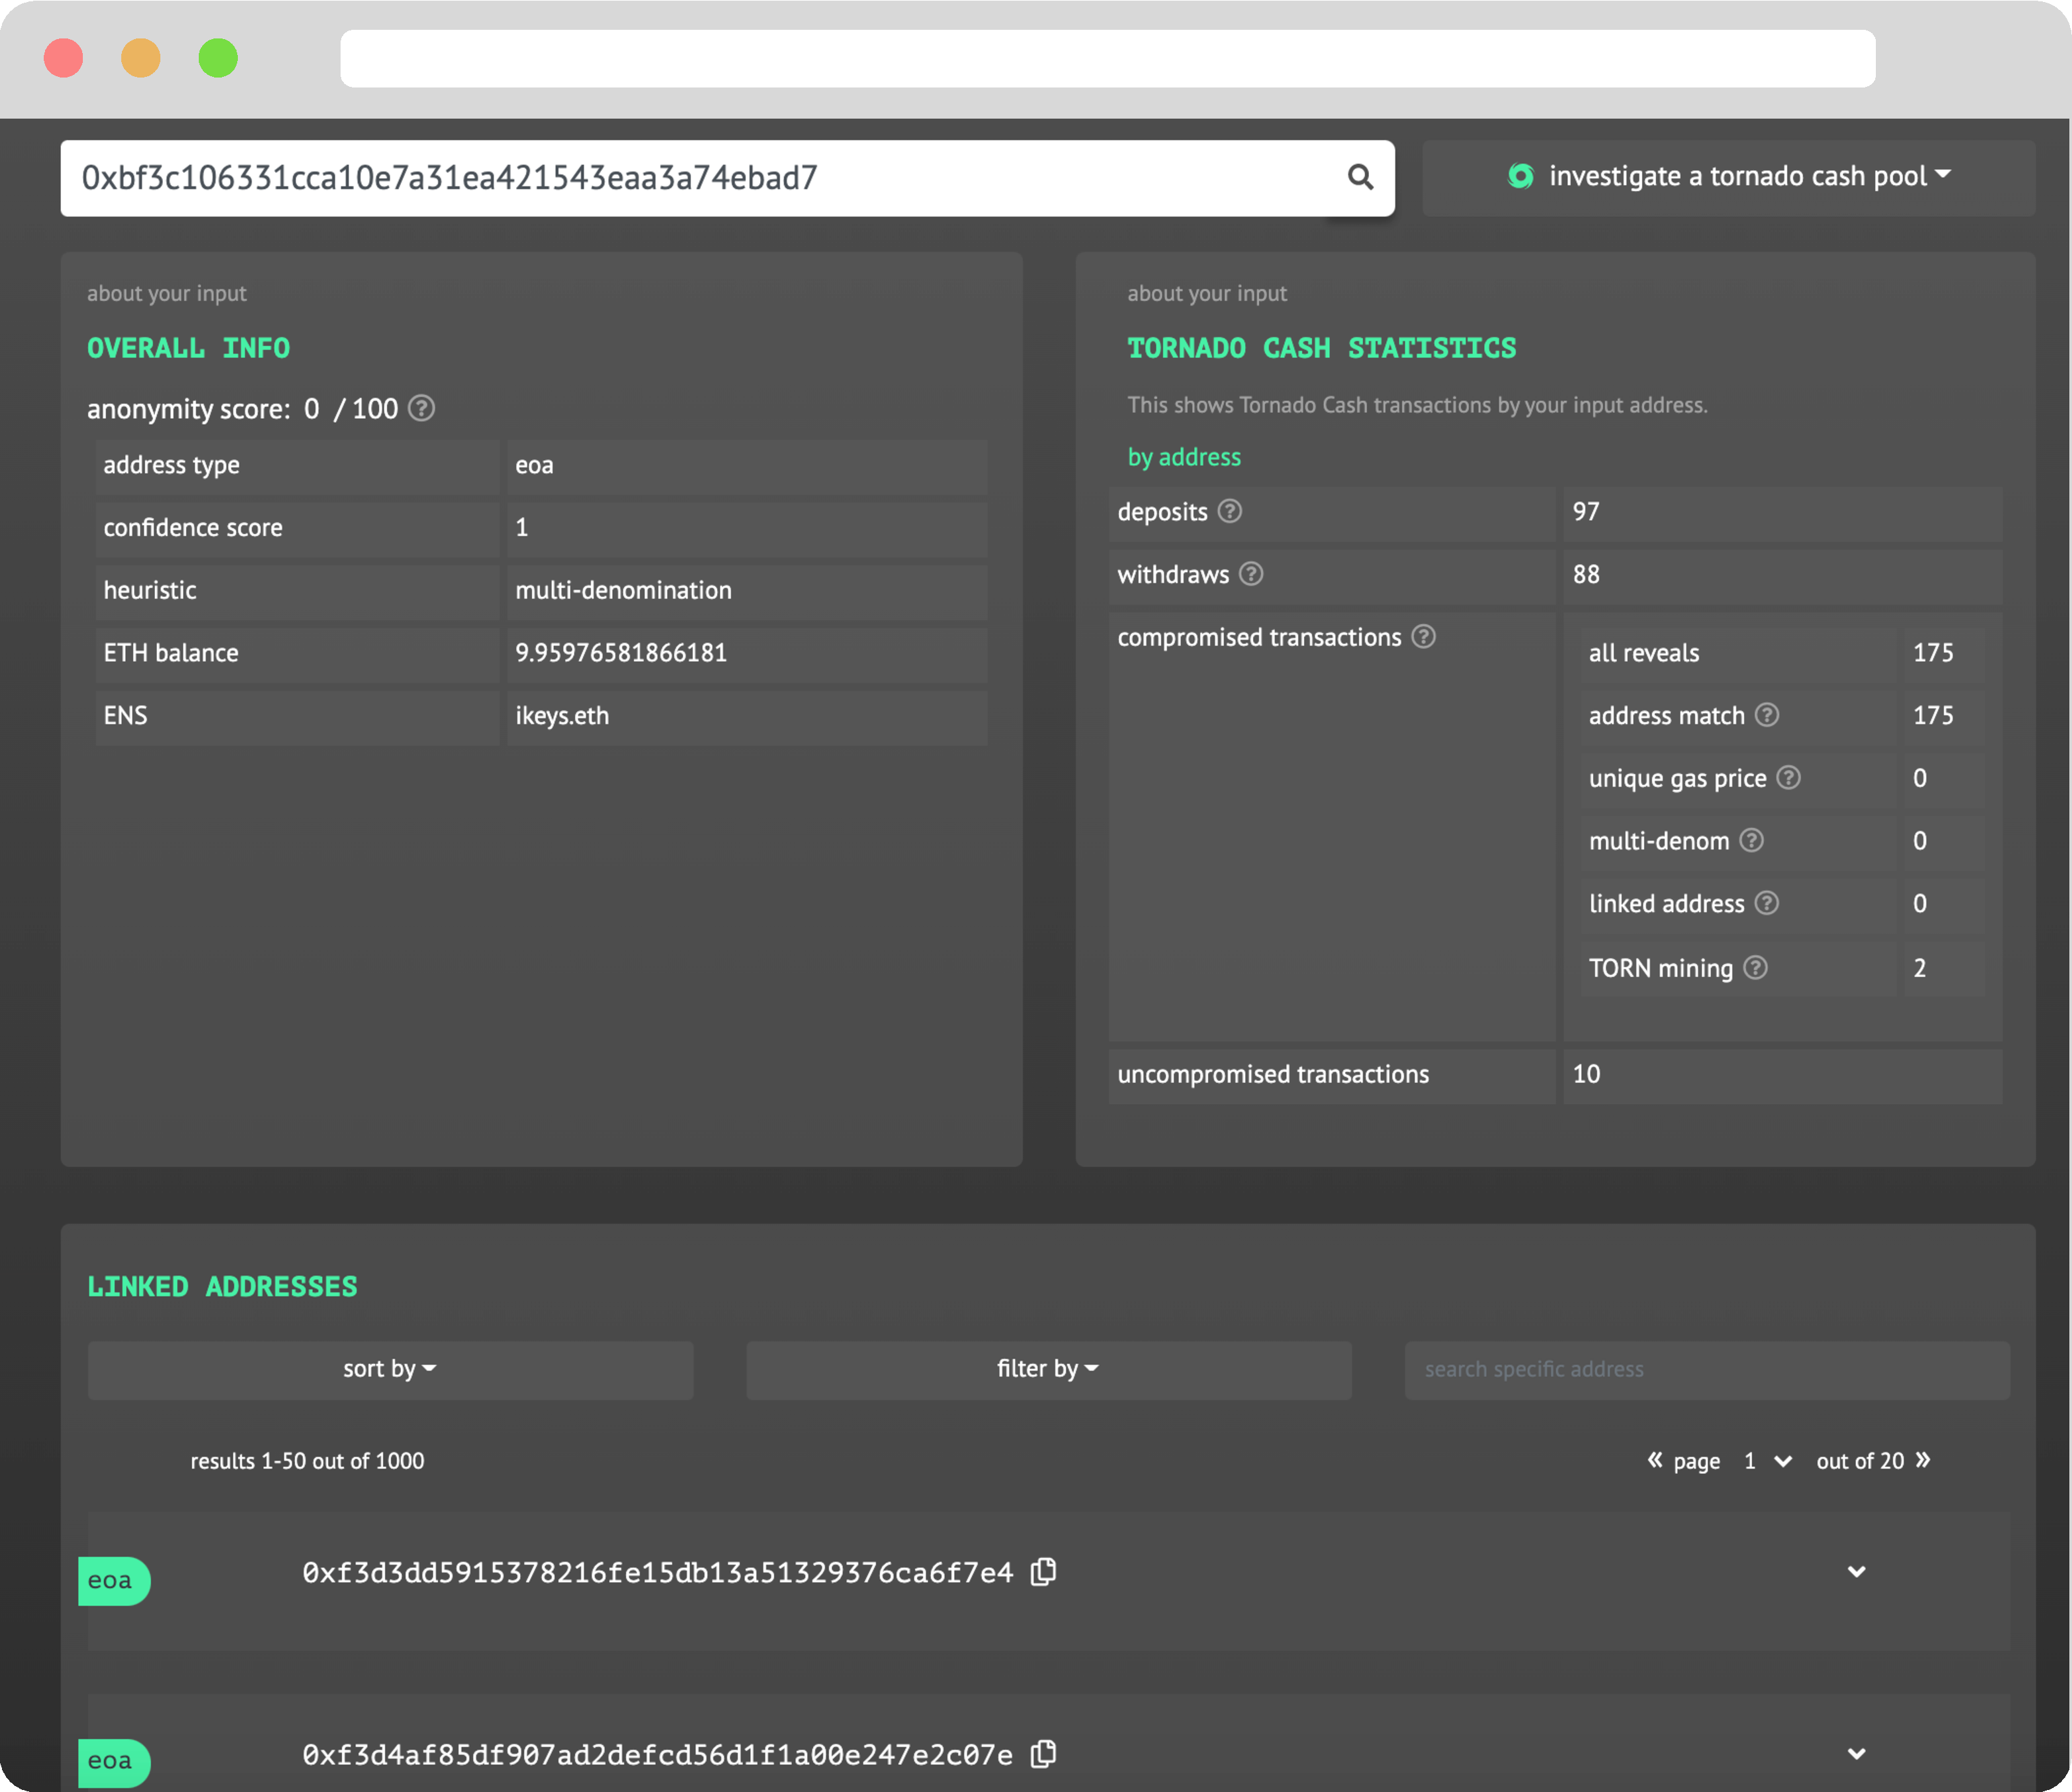
\includegraphics[width=\linewidth]{figures/demo.pdf}
\caption{Tutela interface when searching an Ethereum address. This address is also a Tornado Cash user.}
\label{fig:demo}
\end{figure}

We summarize the main functionalities shown in Figure~\ref{fig:demo}.

\section{Data and Setup}

TODO

\section{Ethereum Heuristics}

\subsection{Deposit Address Reuse}

\subsection{Diff2Vec}

\section{Tornado Cash Heuristics}

\subsection{Address Match}

\subsection{Unique Gas Price}

\subsection{Multiple Denomination}

\subsection{Interaction History}

\section{Analysis}

TODO. This is where most of the heavy lifting needs to happen.

\section{Discussion}

\subsection{Limitations}

\subsection{Extensions}

\subsection{Broader Impact}

\bibliography{whitepaper}
\bibliographystyle{acl_natbib}

\end{document}
